\documentclass[10pt]{academydoc}
\usepackage{siunitx}
\usepackage{mathptmx}
\usepackage{bm}
\usepackage[backend=bibtex, style=ieee, sorting=none]{biblatex}
\usepackage{amsmath}
\bibliography{citations.bib}

\newcolumntype{Y}{>{\centering\arraybackslash}X}

\newcommand{\rgbequal}[0]{%
    $R{=}G{=}B$%
    \ignorespaces
}%

\pagestyle{plain}


% Set Document Details
\doctype{tb} % spec, proc, tb (Specification, Procedure, Technical Bulletin)
\docname{Derivation of the ACES white point \\CIE chromaticity coordinates}
\altdocname{Derivation of the ACES white point CIE chromaticity coordinates}
% Sets the document name used in header - usually an abbreviated document title
\docnumber{TB-2018-001}
\committeename{Academy Color Encoding System (ACES) Project}
\docdate{June 15, 2018}
\summary{
This document describes the derivation of the white point CIE chromaticity coordinates used in various ACES encodings including ACES2065-1, ACEScg, ACESproxy, ACEScc and details of why the chromaticity coordinates were chosen.
}

% Document Starts Here
\begin{document}

\maketitle

% This file contains the content for the Notices
\prelimsectionformat	% Change formatting to that of "Notices" section
\chapter[Notices]{\uppercase{Notices}}
%% Modify below this line %%

\copyright\the\year{} Academy of Motion Picture Arts and Sciences (A.M.P.A.S.). All rights reserved. This document is provided to individuals and organizations for their own internal use, and may be copied or reproduced in its entirety for such use. This document may not be published, distributed, publicly displayed, or transmitted, in whole or in part, without the express written permission of the Academy.

The accuracy, completeness, adequacy, availability or currency of this document is not warranted or guaranteed. Use of information in this document is at your own risk. The Academy expressly disclaims all warranties, including the warranties of merchantability, fitness for a particular purpose and non-infringement.

Copies of this document may be obtained by contacting the Academy at councilinfo@oscars.org.

``Oscars,'' ``Academy Awards,'' and the Oscar statuette are registered trademarks, and the Oscar statuette a copyrighted property, of the Academy of Motion Picture Arts and Sciences.

% This paragraph is optional.  Comment out if you wish to remove it.
This document is distributed to interested parties for review and comment. A.M.P.A.S. reserves the right to change this document without notice, and readers are advised to check with the Council for the latest version of this document.

% This paragraph is optional.  Comment out if you wish to remove it.
The technology described in this document may be the subject of intellectual property rights (including patent, copyright, trademark or similar such rights) of A.M.P.A.S. or others. A.M.P.A.S. declares that it will not enforce any applicable intellectual property rights owned or controlled by it (other than A.M.P.A.S. trademarks) against any person or entity using the intellectual property to comply with this document.

% This paragraph is optional.  Comment out if you wish to remove it.
Attention is drawn to the possibility that some elements of the technology described in this document, or certain applications of the technology may be the subject of intellectual property rights other than those identified above. A.M.P.A.S. shall not be held responsible for identifying any or all such rights. Recipients of this document are invited to submit notification to A.M.P.A.S. of any such intellectual property of which they are aware.

\vspace{10pt}
These notices must be retained in any copies of any part of this document. \newpage
% This file contains the content for the Revision History and 
\prelimsectionformat	% Change formatting to that of "Notices" section
\chapter{Revision History}
%% Modify below this line %%

\begin{tabularx}{\linewidth}{|l|l|X|}
    \hline
    Version & Date       & Description \\ \hline
    1.0     & xx/xx/2017 & Initial Version \\ \hline
    &   &   \\ \hline
    &   &   \\ \hline
    &   &   \\ \hline
\end{tabularx}

\vspace{0.25in} % <-- DO NOT REMOVE
\chapter{Related Academy Documents} % <-- DO NOT REMOVE
\begin{tabularx}{\linewidth}{|l|X|}
    \hline
    Document Name & Description \\ \hline
     & \\ \hline
     & \\ \hline
     & \\ \hline
     & \\ \hline
     & \\ \hline
\end{tabularx} \newpage

\tableofcontents \newpage

% This file contains the content for the Introduction
\unnumberedformat	    % Change formatting to that of "Introduction" section
\chapter{Introduction} 	% Do not modify section title
%% Modify below this line %%
ACES 1.0 includes thirteen Output Transforms that can be broadly characterized as applying to four different display types used in various configurations. (Table \ref{odt-display-types-table}) The display types include digital cinema projectors typically used in digital intermediate, motion picture mastering, and theatrical exhibition, standard dynamic range (SDR) broadcast displays used in editorial and on-set preview applications, high dynamic range (HDR) broadcast displays used in mastering an exhibition of HDR content, and computer desktop monitors such as those typically used in the creation of computer generated visual effects (VFX).

\begin{table}[ht!]
\centering
\begin{tabular}{cc}
\textbf{Output Transform (Short Name)}                              & \textbf{Display Type}                               \\ \hline
\multicolumn{1}{|l|}{ACES 1.0 Output - P3-DCI}                      & \multicolumn{1}{l|}{Digital Cinema Projector (SDR)} \\ \hline
\multicolumn{1}{|l|}{ACES 1.0 Output - P3-D60}                      & \multicolumn{1}{l|}{Digital Cinema Projector (SDR)} \\ \hline
\multicolumn{1}{|l|}{ACES 1.0 Output - DCDM}                        & \multicolumn{1}{l|}{Digital Cinema Projector (SDR)} \\ \hline
\multicolumn{1}{|l|}{ACES 1.0 Output - DCDM (P3 gamut clip)}        & \multicolumn{1}{l|}{Digital Cinema Projector (SDR)} \\ \hline
\multicolumn{1}{|l|}{ACES 1.0 Output - Rec.709}                     & \multicolumn{1}{l|}{SDR Broadcast Monitor}          \\ \hline
\multicolumn{1}{|l|}{ACES 1.0 Output - Rec.709 (D60 sim.)}          & \multicolumn{1}{l|}{SDR Broadcast Monitor}          \\ \hline
\multicolumn{1}{|l|}{ACES 1.0 Output - Rec.2020}                    & \multicolumn{1}{l|}{SDR Broadcast Monitor}          \\ \hline
\multicolumn{1}{|l|}{ACES 1.0 Output - P3-D60 ST2084 (1000 nits)}   & \multicolumn{1}{l|}{HDR Broadcast Monitor}          \\ \hline
\multicolumn{1}{|l|}{ACES 1.0 Output - P3-D60 ST2084 (2000 nits)}   & \multicolumn{1}{l|}{HDR Broadcast Monitor}          \\ \hline
\multicolumn{1}{|l|}{ACES 1.0 Output - P3-D60 ST2084 (4000 nits)}   & \multicolumn{1}{l|}{HDR Broadcast Monitor}          \\ \hline
\multicolumn{1}{|l|}{ACES 1.0 Output - Rec.2020 ST2084 (1000 nits)} & \multicolumn{1}{l|}{HDR Broadcast Monitor}          \\ \hline
\multicolumn{1}{|l|}{ACES 1.0 Output - sRGB}                        & \multicolumn{1}{l|}{Desktop Computer Display}       \\ \hline
\multicolumn{1}{|l|}{ACES 1.0 Output - sRGB (D60 sim.)}             & \multicolumn{1}{l|}{Desktop Computer Display}       \\ \hline
\end{tabular}
\caption[ACES 1.0 Output Device Transforms and Display Types]{ACES 1.0 Output Device Transforms and Display Types}
\label{odt-display-types-table}
\end{table}

The output device to be used with any particular device depends on the detailed configuration of that device.  This document is intended to be practical guide help end-users determine the proper ACES output transform to be used the configuration, workflow, and intended usage.  This document is intended to cover a series of common use cases.  There may be valid uses of the ACES output transforms that fall outside of the scope of this document.

% This file contains the content for the Scope
\cleardoublepage
\numberedformat	
\chapter{Scope} 	% Do not modify section title
%% Modify below this line %%

This document describes the derivation of the ACES white point CIE chromaticity coordinates and details of why the chromaticity coordinates were chosen.  This document includes links to an example Python implementation of the derivation and an iPython notebook intended to help readers reproduce the referenced values.

This document is primarily intended for those interested in understanding the details of the technical specification of ACES and the history of its development. The definition of a color space encoding's white point chromaticity coordinates is one important factor in the definition of a color managed system. The white point used in various ACES encodings does not dictate the creative white point of images created or mastered using the ACES system. It exists to enable accurate conversion to and from the other color encodings such as CIE XYZ.  The proper usage of the ACES white point in conversion, mastering, or reproduction are beyond the scope of this document.  For example, the proper usage of the ACES white point in encoding scene colorimetry in ACES2065-1 is detailed in P-2013-001 \cite{idt}.  

% This section contains the content for the References
\numberedformat
\chapter{References}
The following standards, specifications, articles, presentations, and texts are referenced in this text:
%% Modify below this line %%

SMPTE ST 2065-1:2012, Academy Color Encoding Specification (ACES)

SMPTE ST 2084:2014, Dynamic Range Electro-Optical Transfer Function of Mastering Reference Displays

ITU-R Rec. BT.709, Parameter values for the HDTV standards for production and international programme exchange 

ITU-R Rec. BT.1886, Reference electro-optical transfer function for flat panel displays used in HDTV studio production

ITU-R Rec. BT.2020, Parameter values for ultra-high definition television systems for production and international programme exchange

ITU-R Rec. BT.2100, Image parameter values for high dynamic range television for use in production and international programme exchange

IEC 61966-2-1, Multimedia systems and equipment -- Colour measurement and management -- Part 2-1: Colour management -- Default RGB colour space -- sRGB
% This file contains the content for a main section
\newpage
\regularsectionformat
%% Modify below this line %%
\chapter{Derivation of CIE chromaticity coordinates}
\label{chap:dervation}

The CIE xy chromaticity coordinates of the ACES white point are specified in SMPTE ST 2065-1:2012 as $x=0.32168$ $y=0.33767$ \cite{SMPTE20651}. The ACES white point chromaticity coordinates are derived using the following procedure:

\begin{enumerate}
    \item Calculate the CIE Daylight spectral power distribution for a Correlated Color Temperature (CCT) of \SI[mode=text]{6000}{\kelvin} over the wavelength intervals \SI[mode=text]{300}{\nm} to \SI[mode=text]{830}{\nm} in \SI[mode=text]{1}{\nm} increments as specified in CIE 15:2004 Section 3.1 \cite{CIE152004}
    \item Calculate the CIE 1931 XYZ tristimulus values of the spectral power distribution as specified in CIE 15:2004 Section 7.1 \cite{CIE152004}
    \item Convert the CIE XYZ values to CIE xy chromaticity coordinates as specified in CIE 15:2004 Section 7.3 \cite{CIE152004}
    \item Round the CIE xy chromaticity coordinates to 5 decimal places
\end{enumerate}

An implementation of the procedure described above can be found at: \\ \url{https://github.com/ampas/aces-dev/tree/master/documents/python/TB-2018-001/aces_wp.py}
% This file contains the content for a main section
\regularsectionformat
%% Modify below this line %%
\chapter{Discussion}
\label{chap:discussion}

\section{Comparison of the ACES white point and CIE \texorpdfstring{D\textsubscript{60}}{D60}}
\label{sec:comp}
Frequently, the white point associated with various ACES encodings is said to be `D\textsubscript{60}' \cite{autodesk,bmforum,acescentralD60}. This shorthand notation has sometimes led to confusion for those familiar with the details of how the chromaticity coordinates of the CIE D series illuminants are calculated \cite{notD60}.  The chromaticity coordinates of any CIE D series illuminant can be calculated using the equations found in Section 3 of CIE 15:2004 and reproduced in Equation~\ref{eq:xyeq} \cite{CIE152004}.

\begin{floatequ}[!ht]
    \begin{alignat*}{2}
    & y_{D} && = -3.000x_{D}^{2}+2.870x_{D}-0.275 \\
    & x_{D} && =
        \begin{dcases}
            0.244063+0.09911{\frac {10^{3}}{T}}+2.9678{\frac {10^{6}}{T^{2}}}-4.6070{\frac {10^{9}}{T^{3}}} \qquad & 4,000\ \mathrm {K} \leq T\leq 7,000\ \mathrm {K} \\
            0.237040+0.24748{\frac {10^{3}}{T}}+1.9018{\frac {10^{6}}{T^{2}}}-2.0064{\frac {10^{9}}{T^{3}}} \qquad & 7,000\ \mathrm {K} < T\leq 25,000\ \mathrm {K}
        \end{dcases}
    \end{alignat*}
    
    \captionsetup{width=.75\textwidth}
    \caption{Calculation of CIE xy from CCT for CIE Daylight}
    \label{eq:xyeq}
\end{floatequ}

The CIE has specified four canonical daylight illuminants (D\textsubscript{50}, D\textsubscript{55}, D\textsubscript{65} and D\textsubscript{75}) \cite{CIE152004}.  Contrary to what the names might imply, the correlated color temperature (CCT) values of these four canonical illuminants are not the nominal CCT values of \SI[mode=text]{5000}{\kelvin}, \SI[mode=text]{5500}{\kelvin}, \SI[mode=text]{6500}{\kelvin}, and \SI[mode=text]{7500}{\kelvin}.  For instance, CIE D\textsubscript{65} does not have a CCT of \SI[mode=text]{6500}{\kelvin} but rather a CCT temperature of approximately \SI[mode=text]{6504}{\kelvin} \cite{wyszecki1982color}.  
The exact CCT values differ from the nominal CCT values due to a 1968 revision to $c_2$, the second radiation constant in Planck's blackbody radiation formula \cite{Durieux1970}.  When the value of $c_2$ was changed from 0.014380 to 0.014388, it altered the CIE xy location of the Planckian locus for a blackbody. This small change to the Planckian locus' position relative to the chromaticity coordinates of the established CIE daylight locus had the effect of changing the correlated color temperature of the CIE D series illuminants ever so slightly.  The precise CCT values for the established canonical CIE D series illuminants can be determined by applying the equation in Equation~\ref{eq:ccteq} to the nominal CCT values implied by the illuminant name.  The exact CCT values of the canonical daylight illuminants are not whole numbers after the correction factor is applied, but it is common to round their values to the nearest Kelvin.  The CCT values of the CIE canonical daylight illuminants before the 1968 change to $c_2$, after the 1968 change, and rounded to the nearest Kelvin can be found in Table~\ref{tab:d_cct}. 

\begin{floatequ}[!ht]
\begin{equation}
    CCT_{new} = CCT\times \frac{1.4388}{1.4380}
\end{equation}
    \captionsetup{width=.75\textwidth}
    \caption{Conversion of nominal pre-1968 CCT to post-1968 CCT}
    \label{eq:ccteq}
\end{floatequ}

\begin{table}[!ht]
    \centering
    \begin{tabularx}{.97\linewidth}{|Y|Y|Y|Y|}
    \hline
    \textbf{CIE D} & \textbf{CCT} & \textbf{CCT current} & \textbf{CCT current} \\ [-1.3ex]
    \textbf{Illuminant} & \textbf{before 1968} & \footnotesize{\textbf{(round to 3 decimal places)}} & \footnotesize{\textbf{(round to 0 decimal places)}} \\ \hline
    D\textsubscript{50} & \SI[mode=text]{5000}{\kelvin} & \SI[mode=text]{5002.782}{\kelvin} & \SI[mode=text]{5003}{\kelvin} \\ \hline
    D\textsubscript{55} & \SI[mode=text]{5500}{\kelvin} & \SI[mode=text]{5503.060}{\kelvin} & \SI[mode=text]{5503}{\kelvin} \\ \hline
    D\textsubscript{65} & \SI[mode=text]{6500}{\kelvin} & \SI[mode=text]{6503.616}{\kelvin} & \SI[mode=text]{6504}{\kelvin} \\ \hline
	D\textsubscript{75} & \SI[mode=text]{7500}{\kelvin} & \SI[mode=text]{7504.172}{\kelvin} & \SI[mode=text]{7504}{\kelvin} \\ \hline
    \end{tabularx}
    \captionsetup{width=.75\textwidth}
    \caption{CCT of canonical CIE daylight illuminants \cite{tableValsPython}}
    \label{tab:d_cct}
\end{table}

D\textsubscript{60} is not one of the four CIE canonical daylight illuminants so the exact CCT of such a daylight illuminant could be interpreted to be either approximately \SI[mode=text]{6003}{\kelvin} ($6000 \times \frac{1.4388}{1.4380}$) or \SI[mode=text]{6000}{\kelvin}.  Regardless, the ACES white point chromaticity coordinates derived using the method specified in Section~\ref{chap:dervation} differs from both the chromaticity coordinates of CIE daylight with a CCT of \SI[mode=text]{6003}{\kelvin} and CIE daylight with a CCT of \SI[mode=text]{6000}{\kelvin}.  The chromaticity coordinates of each, rounded to 5 decimal places, can be found in Table~\ref{tab:ciexy}.  As illustrated in Figure~\ref{fig:cieuv}, the chromaticity coordinates of the ACES white point do not fall on the daylight locus nor do they match those of any CIE daylight spectral power distribution.  The positions of the chromaticity coordinates in CIE Uniform Color Space (u$^\prime$v$^\prime$) and the differences from the ACES chromaticity coordinates in $\Delta$u$^\prime$v$^\prime$ can be found in Table~\ref{tab:cieuv}.

\begin{table}[!ht]
    \centering
    \begin{tabularx}{.75\linewidth}{|l|Y|Y|}
    \hline
     & \textbf{CIE $\boldsymbol{x}$} & \textbf{CIE $\boldsymbol{y}$} \\ \hline
    ACES White Point & 0.32168 & 0.33767 \\ \hline
    CIE Daylight 6000K & 0.32169  & 0.33780 \\ \hline
	CIE Daylight 6003K & 0.32163  & 0.33774 \\ \hline
    \end{tabularx}
    \captionsetup{width=.75\textwidth}
    \caption{CIE xy chromaticity coordinates rounded to 5 decimal places \cite{tableValsPython}}
    \label{tab:ciexy}
\end{table}

\begin{table}[!ht]
    \centering
    \begin{tabularx}{.75\linewidth}{|l|Y|Y|Y|}
    \hline
     & \textbf{CIE $\boldsymbol{u^\prime}$} & \textbf{CIE $\boldsymbol{v^\prime}$} & $\boldsymbol{\Delta u^\prime v^\prime}$ \\ \hline
    ACES White Point & 0.20078 & 0.47421 & 0\\ \hline
    CIE Daylight 6000K & 0.20074 & 0.47427 & 0.00008 \\ \hline
	CIE Daylight 6003K & 0.20072 & 0.47423 & 0.00007 \\ \hline
    \end{tabularx}
    \captionsetup{width=.75\textwidth}
    \caption{CIE u$^\prime$v$^\prime$ chromaticity coordinates and $\Delta$u$^\prime$v$^\prime$ from the ACES white point rounded to 5 decimal places \cite{tableValsPython}}
    \label{tab:cieuv}
\end{table}

\begin{figure}[!ht]
    \centering
    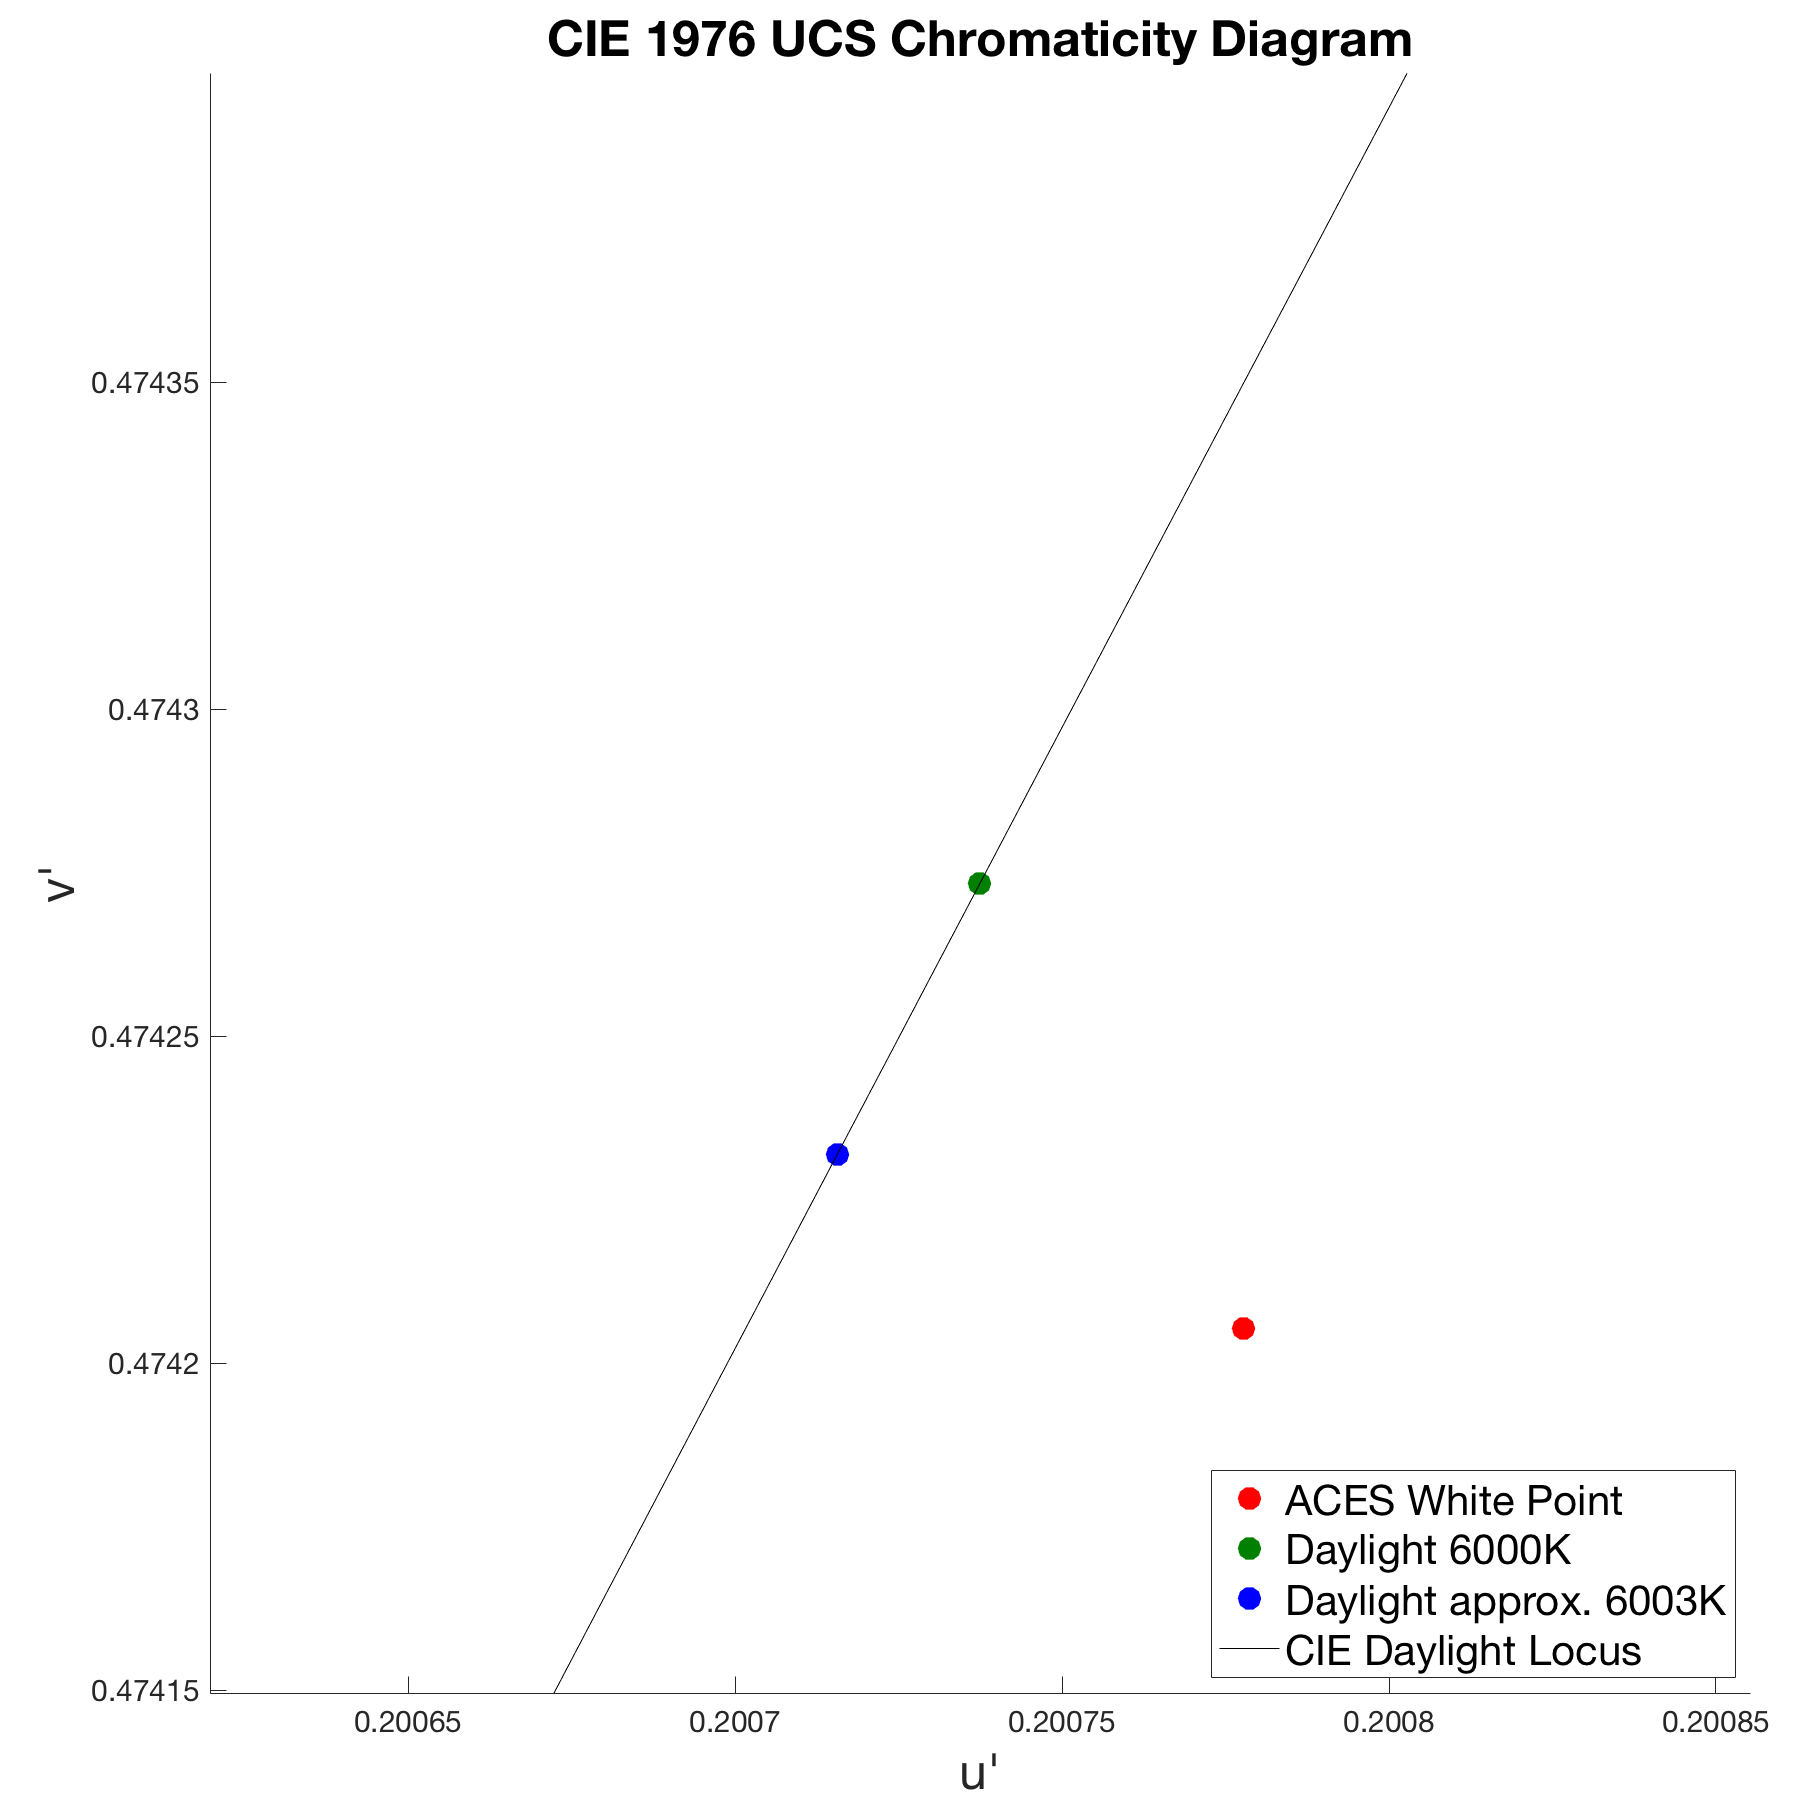
\includegraphics[width=0.5\textwidth]{cieuv.png}
    \caption{CIE UCS diagram with chromaticity coordinates}
    \label{fig:cieuv}
\end{figure}

Although the ACES white point chromaticity is not on either the Planckian locus or the daylight locus, the CCT of its chromaticity can still be estimated.  There are a number of methods for estimating the CCT of any particular set of chromaticity coordinates \cite{robertson1968computation,mccamy1992correlated,hernandez1999calculating,Ohno2014}.  The results of four popular methods can be found in Table~\ref{tab:aceswpcct}.  Each of the methods estimates the CCT of the ACES white point to be very close to \SI[mode=text]{6000}{\kelvin}.

\begin{table}[!ht]
    \centering
    \begin{tabularx}{.9\linewidth}{|Y|Y|}
    \hline
    \textbf{CCT Estimation Method} & \textbf{ACES white point CCT} \\ \hline
    Robertson & \SI[mode=text]{5998.98}{\kelvin} \\ \hline
    Hernandez-Andres & \SI[mode=text]{5997.26}{\kelvin} \\ \hline
    Ohno & \SI[mode=text]{6000.04}{\kelvin} \\ \hline
	McCamy & \SI[mode=text]{6000.41}{\kelvin} \\ \hline
    \end{tabularx}
    \captionsetup{width=.9\textwidth}
    \caption{Estimation of the CCT of the ACES white point rounded to 2 decimal places \cite{tableValsPython}}
    \label{tab:aceswpcct}
\end{table}

\section{Reasons for the ``\texorpdfstring{D\textsubscript{60}}{D60}-like'' white point}
\label{sec:reasonForD60}
The ACES white point was first specified by the Academy's ACES Project Committee in 2008 in Academy Specification S-2008-001.  The details in S-2008-001 were later standardized in SMPTE ST 2065-1:2012.  Prior to the release of the Academy specification the Project Committee debated various aspects of the ACES2065-1 encoding, including the exact white point, for many months.  The choice of the ``D\textsubscript{60}-like'' white point was influenced heavily by discussions centered around viewer adaptation, dark surround viewing conditions, ``cinematic look'', and preference.  In the end, the Committee decided to go with a white point that was close to that of a daylight illuminant but also familiar to those with a film heritage. The white point would later be adopted for use in other encodings used in the ACES system. It is important to note that the ACES white point does not dictate the chromaticity of the reproduction neutral axis.  Using various techniques beyond the scope of this document the chromaticity of the equal red, green and blue (ACES2065-1 \rgbequal) may match the ACES white point, the display calibration white point, or any other white point preferred for technical or aesthetic reasons.

The Committee felt that a white point with a chromaticity similar to that of daylight was appropriate for ACES2065-1.  However, the exact CCT of the daylight was in question.  Some felt D\textsubscript{55} was a reasonable choice given its historical use as the design illuminant for daylight color negative films.  Others felt D\textsubscript{65} would be good choice given its use in television and computer graphics as a display calibration white point.  Because the exact white point chromaticity would not prohibit users from achieving any reproduction white point, the Committee ultimately decided to use the less common CCT of \SI[mode=text]{6000}{\kelvin}.  This choice was based on an experiment to determine the reproduction chromaticity of projected color print film, the relative location of the white point compared to other white points commonly used in digital systems, and the general belief that imagery reproduced with the white point felt aesthetically ``cinematic''.

The projected color print film experiment involved simulating the exposure of a spectrally non-selective (neutral) gray scale onto color negative film, printing that negative onto a color print film, then projecting the color film onto a motion picture screen with a xenon-based film projector and measuring the colorimetry off the screen. The result of the experiment found that the CIE xy chromaticity coordinates of a projected LAD patch \cite{pytlak1976simplified,kodakLad} through a film system were approximately $x=0.32170$ $y=0.33568$. Figure~\ref{fig:filmprintthrough} shows a plot of the CIE $u^\prime v^\prime$ chromaticity coordinates of a scene neutral as reproduced by a film system compared to the CIE daylight locus and the ACES white point.  The chromaticity of the film system LAD reproduction was determined to be closest to CIE daylight with the CCT of \SI[mode=text]{6000}{\kelvin} when the differences were calculated in CIE $u^\prime v^\prime$.  A summary of the CIE $u^\prime v^\prime$ differences between CIE daylight at various CCTs and the LAD patch chromaticity are summarized in Table~\ref{tab:lad}.

\begin{figure}[!ht]
    \centering
    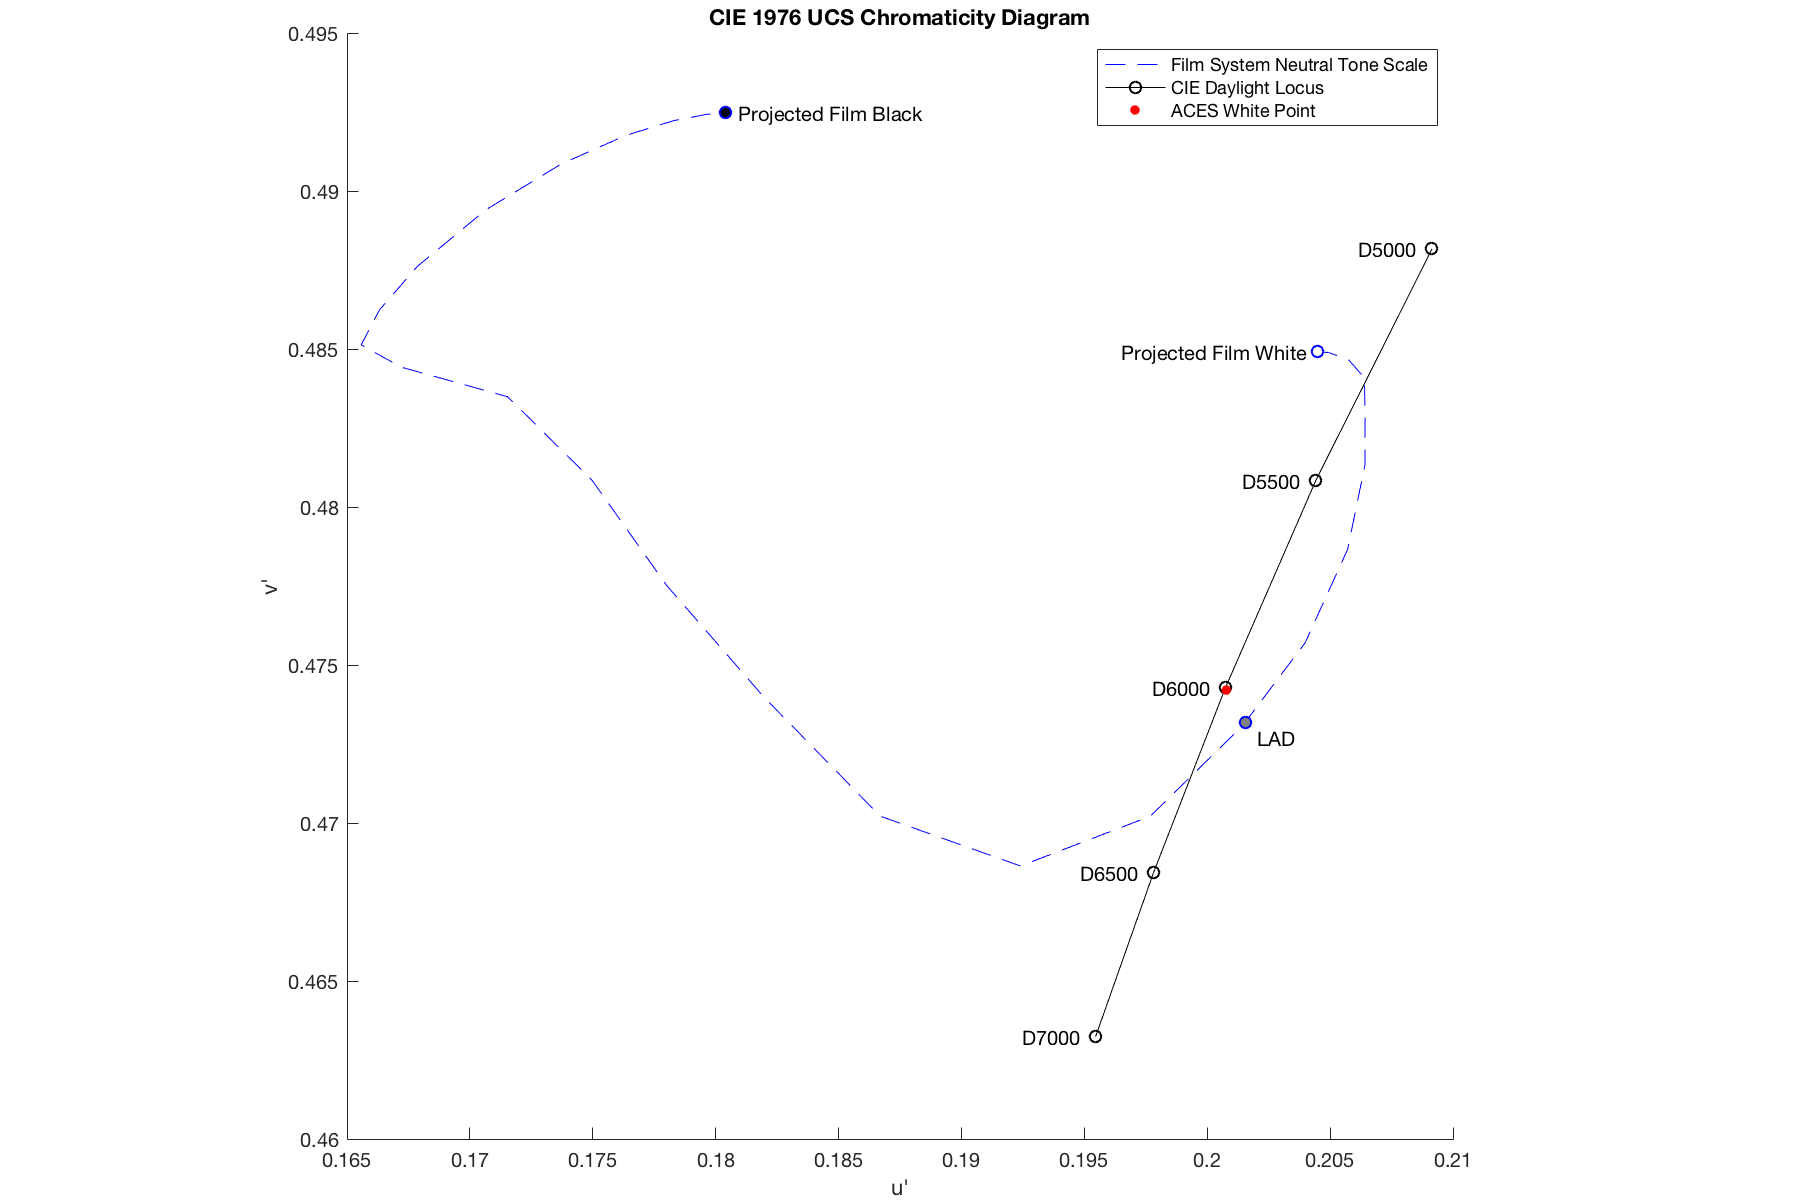
\includegraphics[width=0.85\textwidth]{images/PrintThroughChromaticities.png}
    \caption{Film system print-through color reproduction of original scene neutral scale}
    \label{fig:filmprintthrough}
\end{figure}

\begin{table}[!ht]
    \centering
    \begin{tabularx}{.75\linewidth}{|Y|Y|}
    \hline
    \textbf{Daylight CCT} & $\boldsymbol{\Delta u^\prime v^\prime}$ \textbf{from LAD chromaticity}\\ \hline
		\SI[mode=text]{5500}{\kelvin} & 0.008183 \\ \hline
		\SI[mode=text]{5600}{\kelvin} & 0.006619 \\ \hline
		\SI[mode=text]{5700}{\kelvin} & 0.005112 \\ \hline
		\SI[mode=text]{5800}{\kelvin} & 0.003676 \\ \hline
		\SI[mode=text]{5900}{\kelvin} & 0.002354 \\ \hline
		\SI[mode=text]{6000}{\kelvin} & 0.001360 \\ \hline
		\SI[mode=text]{6100}{\kelvin} & 0.001448 \\ \hline
		\SI[mode=text]{6200}{\kelvin} & 0.002442 \\ \hline
		\SI[mode=text]{6300}{\kelvin} & 0.003627 \\ \hline
		\SI[mode=text]{6400}{\kelvin} & 0.004836 \\ \hline
		\SI[mode=text]{6500}{\kelvin} & 0.006035 \\ \hline
    \end{tabularx}
    \captionsetup{width=.75\textwidth}
    \caption{CIE $\Delta$u$^\prime$v$^\prime$ difference between projected LAD patch and CIE Daylight CCT chromaticity coordinates round to 6 decimal places \cite{tableValsPython}}
    \label{tab:lad}
\end{table}


\section{Reasons why the ACES white point doesn't match the CIE \texorpdfstring{D\textsubscript{60}}{D60} chromaticity coordinates}
\label{sec:reasonsForDifference}
As discussed in Section~\ref{sec:reasonForD60}, the ACES white point was chosen to be very close to that of CIE Daylight with a CCT of \SI[mode=text]{6000}{\kelvin}.  This raises the question why the CIE chromaticity coordinates of $x=0.32169$ $y=0.33780$ were not used.  The reasoning is somewhat precautionary; at the time, the exact chromaticity coordinates for the ACES white point were being debated, the ACES Project Committee was concerned about the implications the choice of any particular set of chromaticity coordinates could suggest.  

Those new to ACES can often misinterpret the specification of a set of ACES encoding white point chromaticity coordinates as a requirement that the final reproduction neutral axis chromaticity is limited to only that white point chromaticity.  However, as pointed out in Section~\ref{sec:reasonForD60}, the ACES encoding white point does not dictate the chromaticity of the reproduction neutral axis, and regardless of the ACES white point chromaticity, the reproduction neutral axis may match the ACES white point, the display calibration white point, or any other white point preferred for technical or aesthetic reasons.  The ACES white point chromaticity coordinates serve to aid in the understanding and, if desired, conversion of the colorimetry of ACES encoded images to any other encoding including those with a different white point.

Just as the implication of the ACES encoding white point on reproduction can be misunderstood, the ACES Project Committee was also concerned that the ACES encoding white point might have unintended implications for image creators. Specifically, the Committee was concerned that the choice of a set of chromaticity coordinates that corresponded to a source with a defined spectral power distribution might be misunderstood to suggest that only that source could be used to illuminate the scene.  For example, the Committee was concerned if the ACES white point chromaticity was chosen to match that of CIE Daylight with a CCT of \SI[mode=text]{6000}{\kelvin} then \textit{only} scenes photographed under CIE Daylight with a CCT of \SI[mode=text]{6000}{\kelvin} would be compatible with the ACES system.  In reality, ACES does not dictate the source under which movies or television shows can be photographed.  ACES Input Transforms handle the re-encoding of camera images to ACES2065-1 and preserve all the technical and artistic intent behind on-set lighting choices.  

For these reasons as well as an abundance of caution, the ACES Project Committee decided it would be best to use a set of chromaticity coordinates very near those of CIE Daylight with a CCT of \SI[mode=text]{6000}{\kelvin} but not exactly those of any easily calculated spectral power distribution.

\end{document}